\chapter{Boosted Decision Trees}
\label{chap:bdt}

This chapter descibes the boosted decision tree algorithm and its use
in the VBF \hwwlnln analysis.

\section{What is a boosted decision tree?}

Boosted decision trees (BDTs) fall into a class of algorithms called machine learning
algorithms. In these algorithms, a computer constructs a model of the
relationship between independent variables, \vect{x}, and some
dependent variable, $y$, in a process called training. These algorithms can
be used for classification of objects that fall into different classes
(ie, signal vs. background) or for regression in the case of a
continuously-distributed, real-valued $y$. Machine
learning techniques, and in particular decision trees, are increasingly used in
particle physics for particle identification and event
classification~\cite{bib:Roe:2004na}. At the LHC, BDTs have been used by both
CMS and ATLAS (references). 

\section{Decision tree learners}

A decision tree is a sequence of selection cuts on the independent
variables, which is shown schematically in
Fig~\ref{chap:bdt:fig:bdt_schem}. In order to grow a decision tree, a
training set of events with known \vect{x} and $y$~ is used to
construct the model $F(\boldsymbol{x})=y$.
In the case of the VBF analysis, there are two classes, signal,
assigned to a numerical value of $y=+1$ and background, $y=-1$, and
the training set is fully simulated Monte Carlo samples. The training
algorithm starts at the root node, and loops through the \vect{x},
finding the variable
that best separates signal and background. The separation is
quantified by the Gini index, given by the sum
$\sum_i p_i(1-p_i)$, where $p_1=\frac{S}{S+B}$ and
$p_2=\frac{B}{S+B}$. This quantity is designed to be minimized if
$p_i=0$ or $p_i=1$, and therefore placing a cut on the variable that
minimizes it yields orthogonal subsamples, called daughter nodes, that are predominantly either
signal or background. The procedure is then repeated at the two
daughter nodes, yielding two more cuts and a total of four
sub-samples. The process is repeated until a minimum number of events 
per node or maximum tree depth is reached. The events in the final
nodes, are assigned a value $y\in \{-1,1\}$, depending on the
majority class in the node.

\begin{figure}[h]
    \centering
    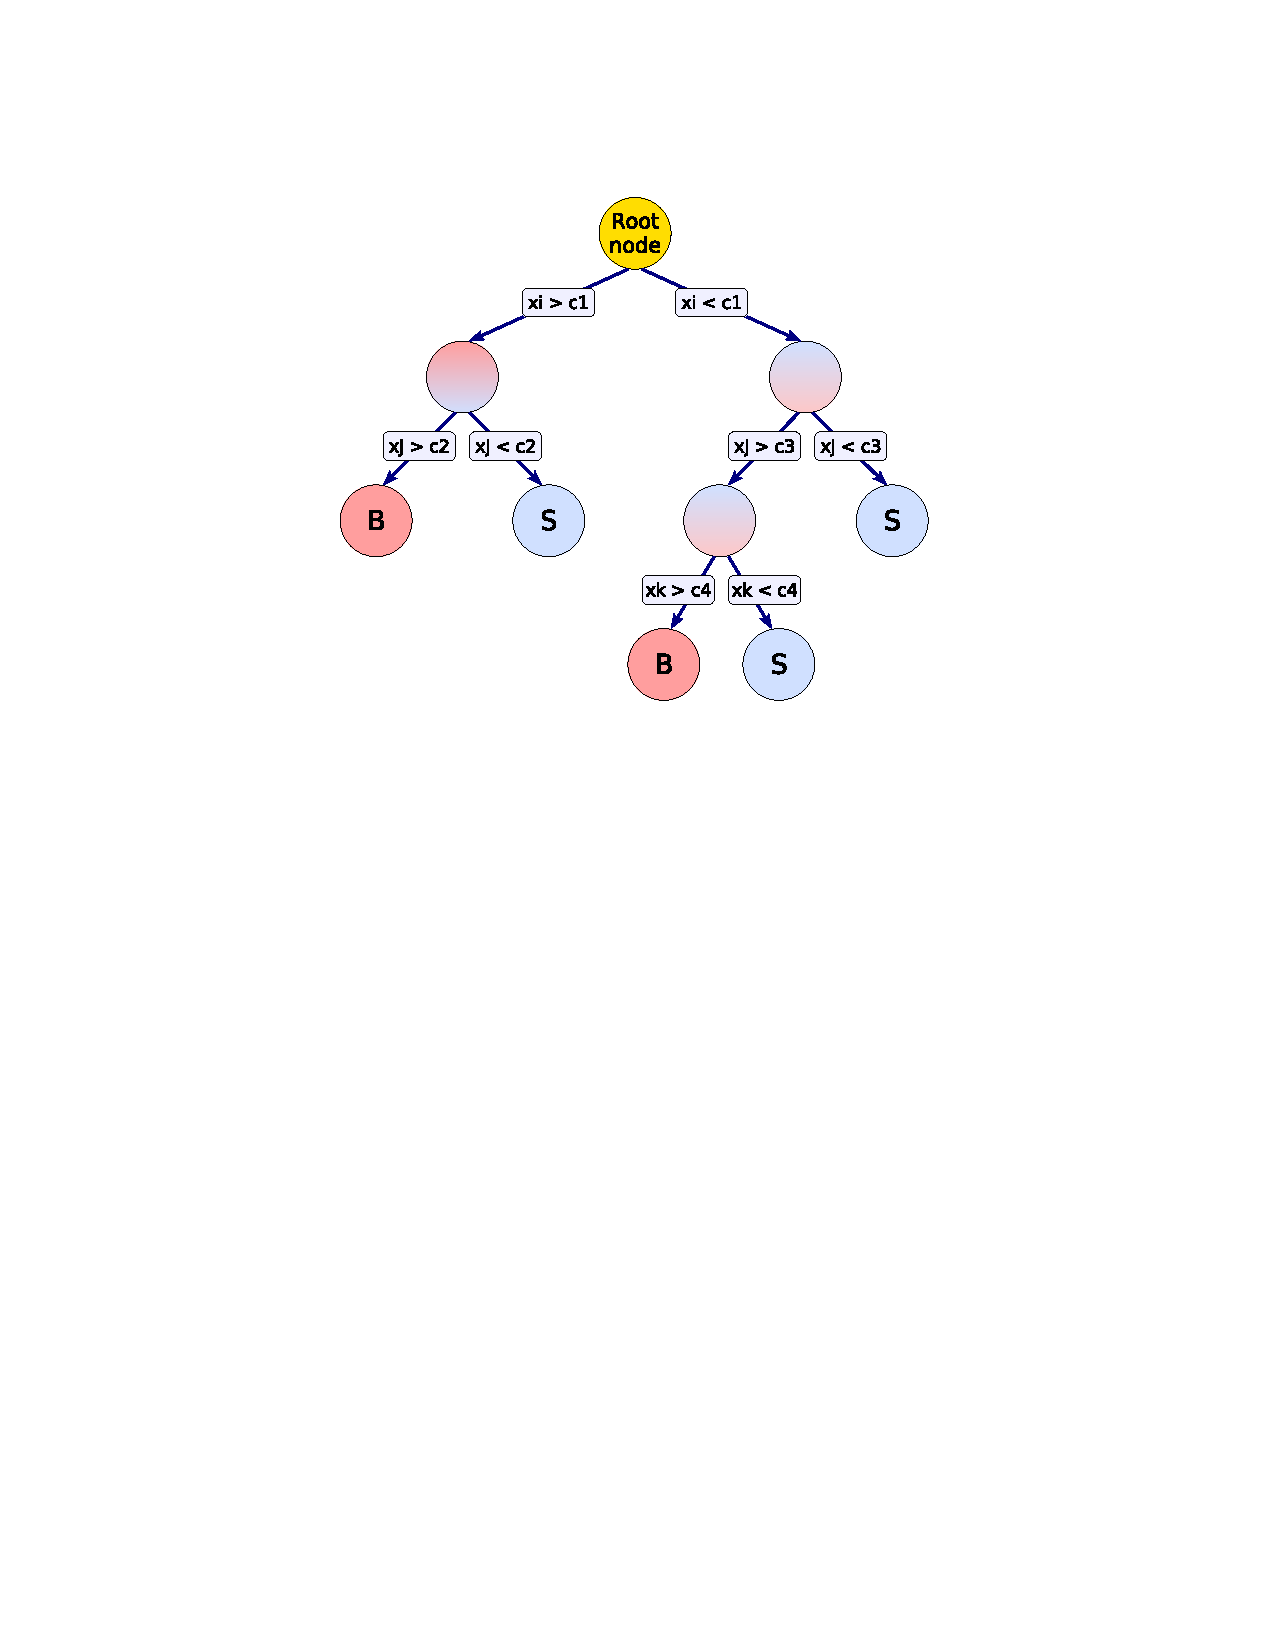
\includegraphics[width=0.90\textwidth]{bdt/bdt_schematic.pdf}
    \caption[Schematic of a boosted decision tree]{Schematic of a boosted decision tree.~\cite{bib:Therhaag:2009dp}}
\label{chap:bdt:fig:bdt_schem}
\end{figure}

The discriminating power of a decision tree classifier lies in its ability to take advantage of
the correlations among the independent variables. To illustrate this,
consider a toy example in which there are two variables, $x_1$ and
$x_2$, plotted for signal and background in
Figure~\ref{chap:bdt:fig:x1_x2}, where the high degree of
correlation is visible. Performing a cut optimization on the two input
distributions, and choosing a signal acceptance working point of
50$\%$ results in the selected box shown in
Figure~\ref{chap:bdt:fig:x1_x2} (a). Because a decision tree is a
sequence of binary cuts, it can be conceptualized as a collection of
boxes in phase space. If the correlations between input variables are
different for signal and background, as is the case for this
example, then the decision tree partitions the phase space into
several signal-rich regions, thereby enhancing the separation
power. This is shown in Figure~\ref{chap:bdt:fig:x1_x2} (b), where the
decision tree picks out a second signal-rich region. Setting the
signal acceptance to the same working point, the decision tree results
in a signal purity, $\frac{S}{S+B}$, of 92$\%$, while the signal purity
with square cuts is 82$\%$.

In general for classification problems, it is uncommon to use a single
decision tree, since this approach is prone to a phenomenon called
overtraining. Overtraining refers to the situation in which the model
constructed during the training process does not generalize to new data
with which a prediction is made. Decision trees are particularly
susceptible to overtraining because the split criteria at
every node depends on all of the parent nodes. Therefore, if there is
a statistical fluctuation or some other systematic noise in the data,
it will be propagated in the growth of the tree. One procedure for
mitigating overtraining is the use of an ensemble of trees, often
called a forest. 

\begin{figure}[h]
    \centering
    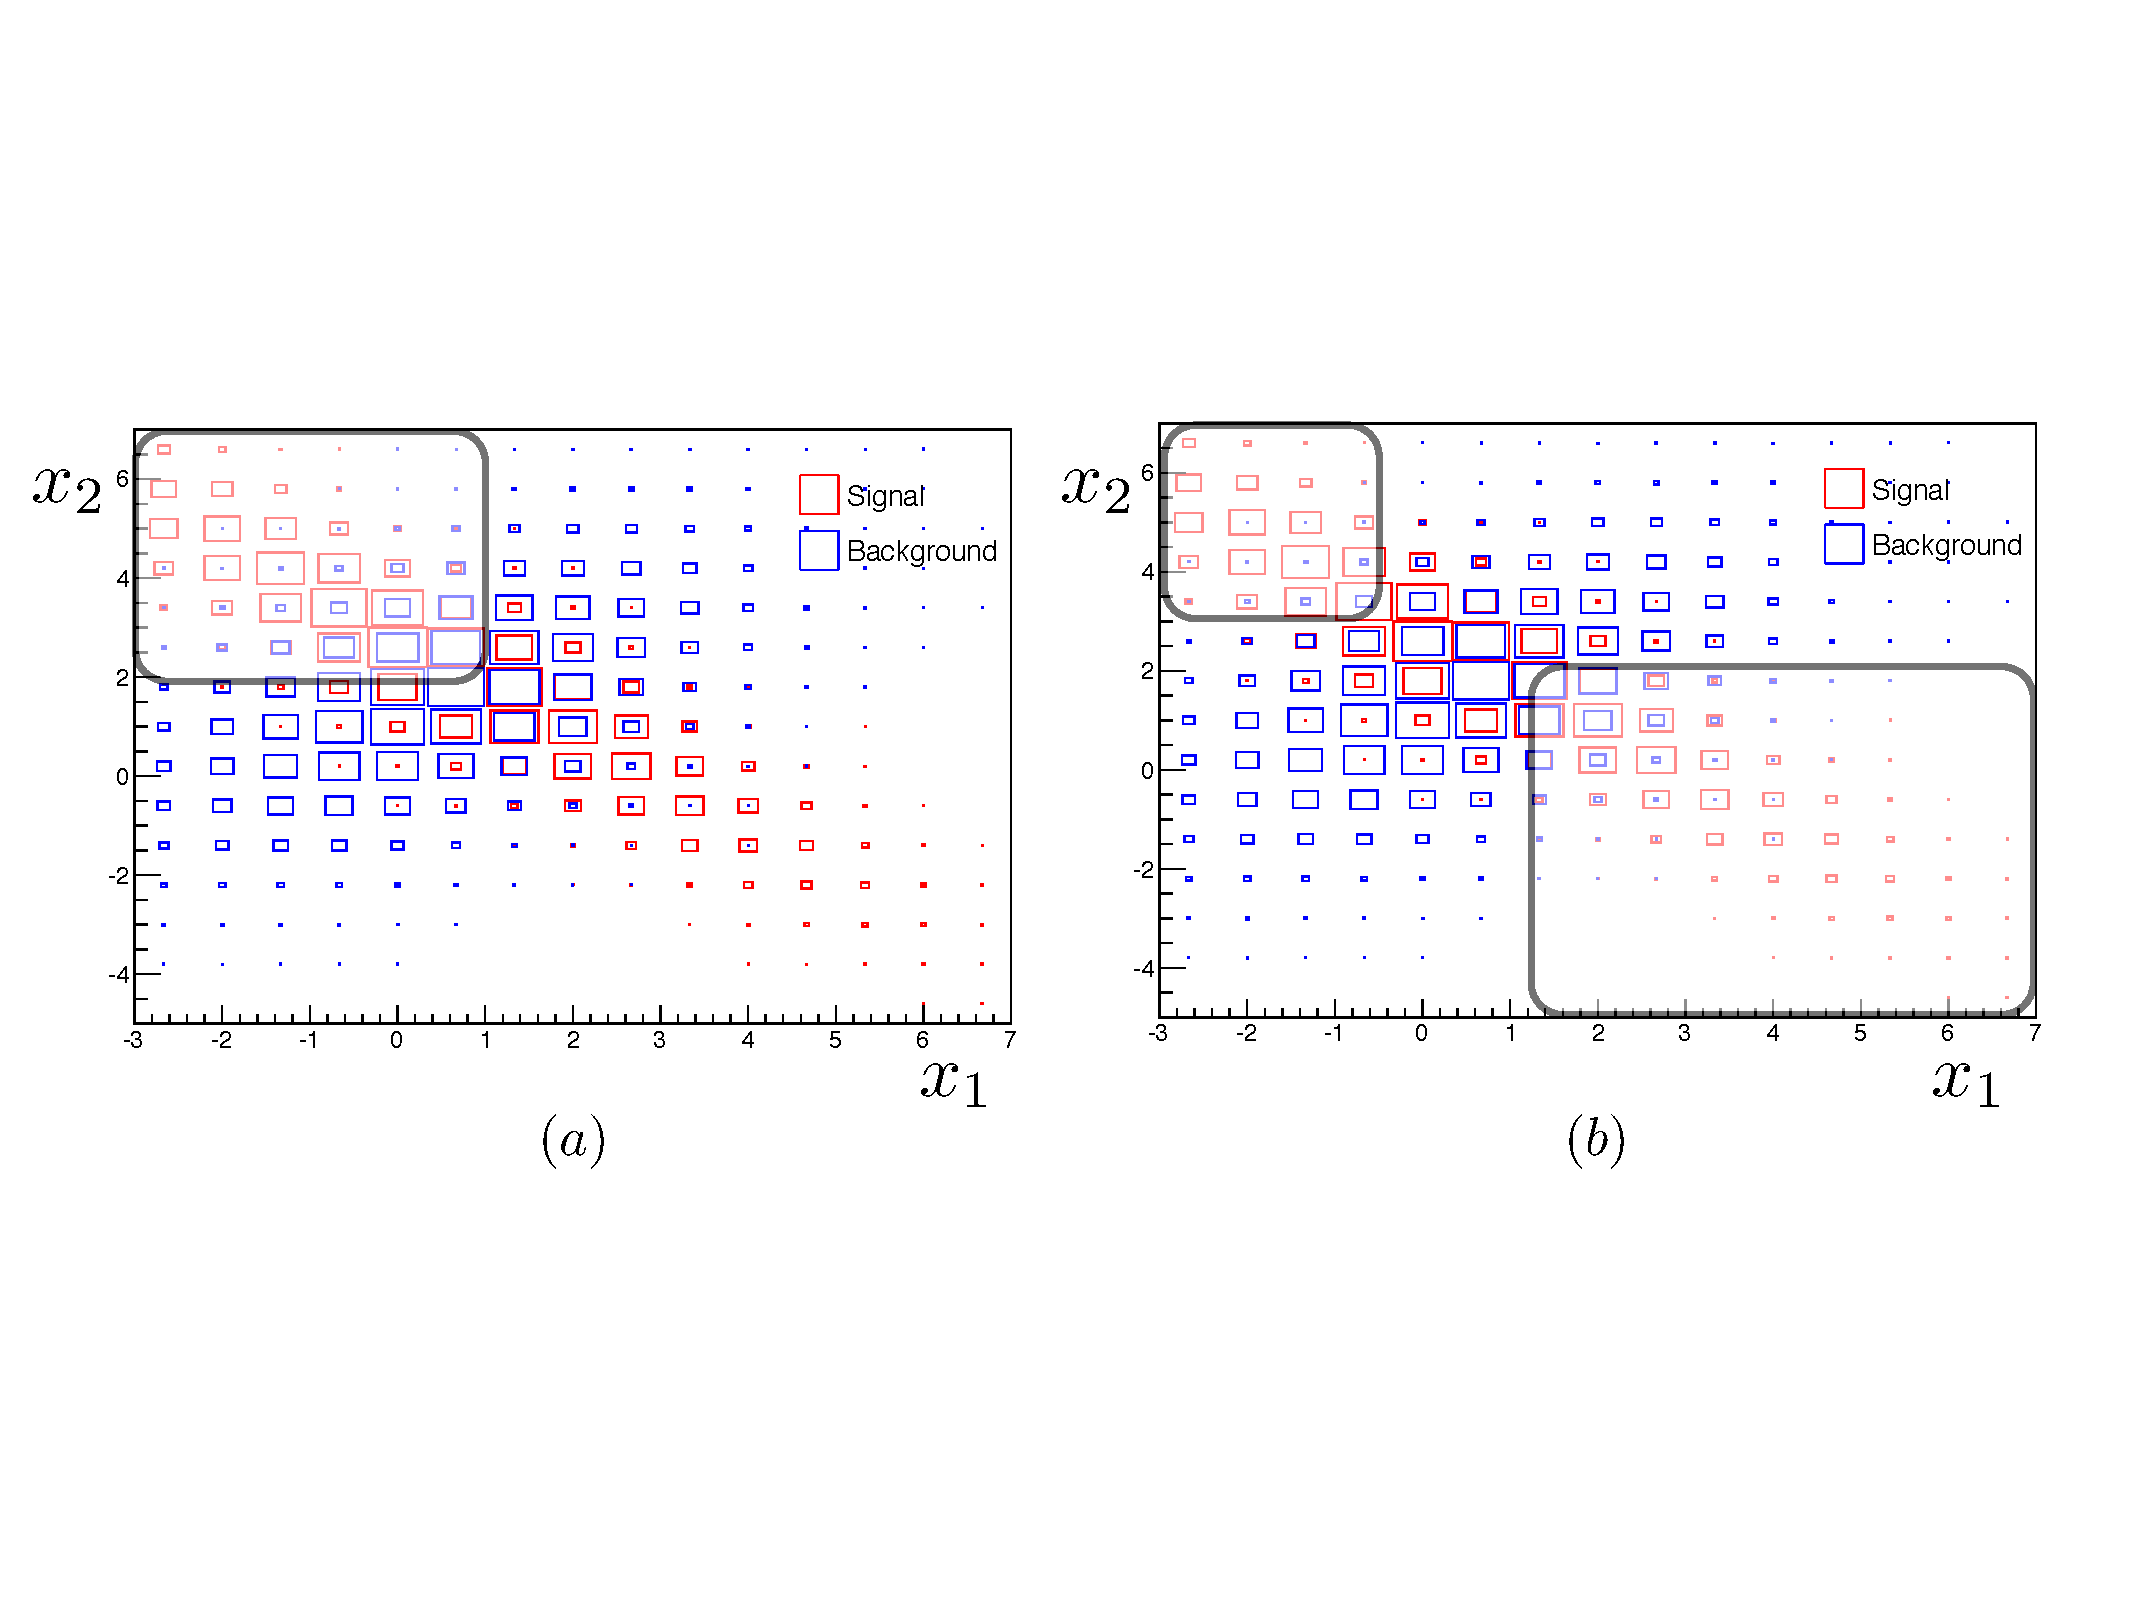
\includegraphics[width=1.0\textwidth]{bdt/x1_vs_x2.pdf}
    \caption[Rectangular cuts vs. decision tree]{Illustration of improved separation power with a decision
    tree in the presence of correlated inputs.}
\label{chap:bdt:fig:x1_x2}
\end{figure}

\section{Boosting}

In the VBF analysis, a procedure known as boosting is used to grow
the decision tree forest. Boosting algorithms grow an ensemble of
``base classifiers'' sequentially, with the training of each classifier
depending on the events that were misclassified by the previous
learner. Events that are misclassified are given a higher weight in
the next iteration in order for the splitting algorithm to focus on
these events. It has been shown that boosting performs well with weak
learners~\cite{bib:Schapire:1990:SWL:83637.83645}, or classifiers that do not perform well
independently. In the case of decision trees, these base classifiers can
be single binary cuts, or a tree with a single node that partitions
the space into two subregions. 

The most commonly used boosting algorthim, proposed by Freund and
Schapire in 1995, is called
\textit{AdaBoost}~\cite{bib:Freund:1995:DGO:646943.712093}. Suppose there
are $N$ events in the training sample, and the target ensemble size is
$M$ trees. In the first iteration of the \textit{AdaBoost} algorithm,
each event is weighted democratically with $w_n^{1} = 1/N$ , and the
base classifer is then built with this training set. For the resulting
classifier, the misclassification fraction is computed as

\begin{equation}
\label{chap:bdt:equation:error_fraction}
    \epsilon_m = \frac{\sum_{n=1}^{N} w_n^m (1-\delta(f_m(\vect{x}_n) -
      y_n))}{\sum_{n=1}^{N} w_n^m}
\end{equation}

\noindent where $n$ indexes the event, $m$ indexes the base classifier, and the
$(1-\delta(f_m(\vect{x}_n) - y_n))$ factor is 0 if the event is
corrected classified and 1 if it is misclassified. The weight for
event $n$ in the subsequent base classifer is then updated according
to the equation

\begin{equation}
\label{chap:bdt:equation:weight_update}
    w_n^{m+1}=w_n^{m}\exp{[\alpha_m (1-\delta(f_m(\vect{x}_n) - y_n))]}
\end{equation}

\noindent where $\alpha_m = \log{(\frac{1-\epsilon_m}{\epsilon_m})}$. If the event
is correctly classified, the weight is unchanged, while for a
misclassified event, the weight in the next training will be larger
and therefore, the training algorithm will place an emphasis on this
event. The final model is expressed as a weighted linear combination
of the base classifiers $F(\vect{x}) = \sgn{\sum_{m=1}^{M} \alpha_m f_m(\vect{x})}$.

%\begin{equation}
%\label{chap:bdt:equation:adaboost_model}
%    F(\vect{x}) = \sgn{\sum_{m=1}^{M} \alpha_m f_m(\vect{x})}
%\end{equation}

The \textit{AdaBoost} algorithm can be reformulated as the
minimization of a loss function~\cite{bib:friedman2000greedy}. The loss function
$L(F(\vect{x},y)$ measures the deviation between the model and the
true value of $y$ in the training set. The specific form of the loss
function depends on the classification problem, and for the \textit{AdaBoost}
algorithm, it can be shown that the loss function is given by

\begin{equation}
\label{chap:bdt:equation:adaboost_loss}
    L(F(\vect{x}),y) = \sum_{n=1}^{N}\exp{(-F(\vect{x}_n)y_n)}.
\end{equation}

\noindent where $y_n \in \{-1,1\}$. Again re-expressing $F(\vect{x})$
as a linear combination of base classifiers

\begin{equation}
\label{chap:bdt:equation:adaboost_loss}
    F(\vect{x}) = \sum_{m=1}^{M} \beta_m f_m(\vect{x}) =
    \sum_{m=1}^{M} \beta_m f(\vect{x};\vect{a}_m)
\end{equation}

\noindent where $\vect{a}_m$ defines the parameters of the base
classifier (in the case of decision trees, the split variables and
values), the task is then to minimimize the loss function with respect
to the weights $\beta_m$ and the parameter vectors $\vect{a}_m$. The
minimization is done numerically with the steepest descent algorithm,
using the derivative of the loss function, and for this reason, this
type of boosting is called ``gradient boosting''. The
\textit{AdaBoost} loss function grows exponentially for large negative
values of $F(\vect{x}_n)y_n$, making it less robust in the face of
statistical or systematic outliers. In the VBF analysis, the loss
function was chosen to be the negative binomial log-likelihood

\begin{equation}
\label{chap:bdt:equation:vbf_loss}
    L(F(\vect{x}),y) = \log (1-\exp{(-F(\vect{x}_n)y_n)}).
\end{equation}

\noindent Since this function grows linearly with $-F(\vect{x}_n)y_n$, it performs
better with noisy data. 

\section{BDT in VBF \hwwlnln}

The VBF \hwwlnln final state is composed many of correlated physics
objects. In selecting a signal-rich phase space region, cuts are
applied on Higgs decay product kinematic distributions, as well as the
jet kinematic distributions characteristic of the VBF production
mode. The general approach with a BDT is to loosen or remove the
rectangular selection cuts and instead train a BDT to find where the
signal lies in phase space. In the case of VBF \hwwlnln, this is expected
to gain in performance over rectangular cuts
because the BDT will find an optimal selection in which the VBF
topological cuts are loosened with tightened $WW$ decay cuts and vice
versa, gaining signal acceptance and improving background rejection. 

\subsection{Optimization}

The software package Toolkit for Multivariate Analysis
(TMVA)~\cite{bib:Therhaag:2009dp} is used for
the implementation of gradient boosting with binary decision trees as the
base classifers. As mentioned above, the negative binomial
log-likelihood loss function is used in this implementation. Although
the TMVA BDT performs quite well out-of-box, optimization was
performed to maximize the expected statistical sensitivity of the
analysis. The BDT was optimized with respect to the BDT inputs, the
tunable parameters of the BDT, and the
preselection cuts applied before after the training. Due to the
computationally intensive nature of training and quantifying the
sensitivity, the minimizations along these DOFs were done sequentially
as opposed to simultaneously. 

The first optimization was done on the
BDT inputs, starting with a set of $50$(?) inputs. The inputs in this
initial set were identified using a combination of physics intuition--
i.e. knowledge of kinematic differences between the dominant
backgrounds and signal-- past experience from the rectangular
cut-based VBF analysis (reference to CONF note), and an exploration of
distributions shown to perform well in other MVA-based Higgs
analyses (reference to H->tautau). The 50 inputs were then used to
train a BDT, and the BDT performance was quantified by computing the
Gaussian significance estimate, $\frac{S}{\sqrt{B}}$, obtained after
cutting on the BDT response distribution at a value corresponding to a
fixed signal acceptance (Koos?). One of the BDT inputs was then pruned
away, and the BDT retrained, yielding a new significance
estimate. This procedure was repeated for each of the 50 inputs,
yielding 50 unique BDTs, each with 49 input distributions. The input
that resulted in the least degradation in the sensitivity was
considered extraneous and removed from the set. This process was
repeated iteratively until the degradation in the sensitivity with
respect to the previous iteration reached some threshold. When the BDT
reached 15 inputs, the figure of merit was changed from the Gaussian
significance estimate to the expected sensitivity computed with the
full statistical framework (described in detail in
Chapter XX) to give a more accurate estimate of the
performance of a given BDT. The BDT inputs were pruned from a set of
50 to a set of 8 before significant losses were observed. The 8 BDT
inputs are described in detail in Chapter YY. 

In the TMVA BDT implementation, there are parameters which can be
adjusted to achieve maximal performance and robustness. The optimal BDT parameter set is a
function of the number of inputs, the number of events in the training
set, and the shapes of the input distributions. There is not a general
prescription for tuning a BDT for a given training set. For this reason, a brute force
optimization was performed on the BDT parameters. The DOFs in the
parameter space were the number of trees in the forest, the maximum
tree depth, the minimum number of events per node, the shrinkage, and
finally the bagging fraction. As discussed above, the forest paradigm
is introduced to reduce the possibility of overtraining. The number of
trees in the forest, the maximum tree depth and the minimum number of
events per node can all be tuned to achieve a model that is not
overfitted, while maintaining the performance of the BDT. The
shrinkage parameter, also known as the learning rate, controls the
degree to which misclassified events are weighted in the boosting
algorithm. Bagging refers to the technique whereby a subset of the
total training set is used in the training of a tree. The events in
the subset are re-sampled with replacement for each tree in the
forest. The bagging fraction parameter in TMVA is the fraction of the
total events that is used in the training subset. For the
optimization, each parameter was scanned, and at each point, the
expected sensivity was computed, using the same technique as the input
optimization. The BDT parameters showing minimal overtraining with
optimal performance are shown in Table~\ref{chap:bdt:tab:bdt_settings}.

\begin{table}
\begin{center}
\begin{tabular}{| l | l |}
    \hline
    Boost algorithm & gradient \\
    Loss function & \begin{math}\log
      (1-\exp{(-F(\vect{x}_n)y_n)})\end{math} \\
    Number of trees & 1000 \\
    Maximum tree depth & 5 \\
    Minimum number of events per node & 1000 \\
    Shrinkage (learning rate) & 0.125 \\
    Bagging fraction & 0.25 \\
    \hline
\end{tabular}
\caption[BDT setting summary.]{Summary of the optimized BDT settings.}
\label{chap:bdt:tab:bdt_settings}
\end{center}
\end{table}

\subsection{Cross-validation and overtraining test}

Classifiers are typically trained and applied on statistically
independent samples. In the VBF analysis, Monte Carlo samples are used
in both the training of the BDT and the prediction of the BDT
response. In order to reduce susceptibility to statistical
fluctuations, all available MC events are used in the final
prediction. To avoid using the same set of events for training and in
the prediction a technique known as cross-validation is used. The full
MC sample is split into two statistically independent subsamples--
even events and odd events. One BDT is trained on even events and
applied to odd events, while one is trained on odd events and applied
to even events. The two BDTs are identical apart from the events in
the training set used to define the BDT. 

\begin{figure}[h]
    \centering
    \subfigure[Overtraining check for BDT 1]{
    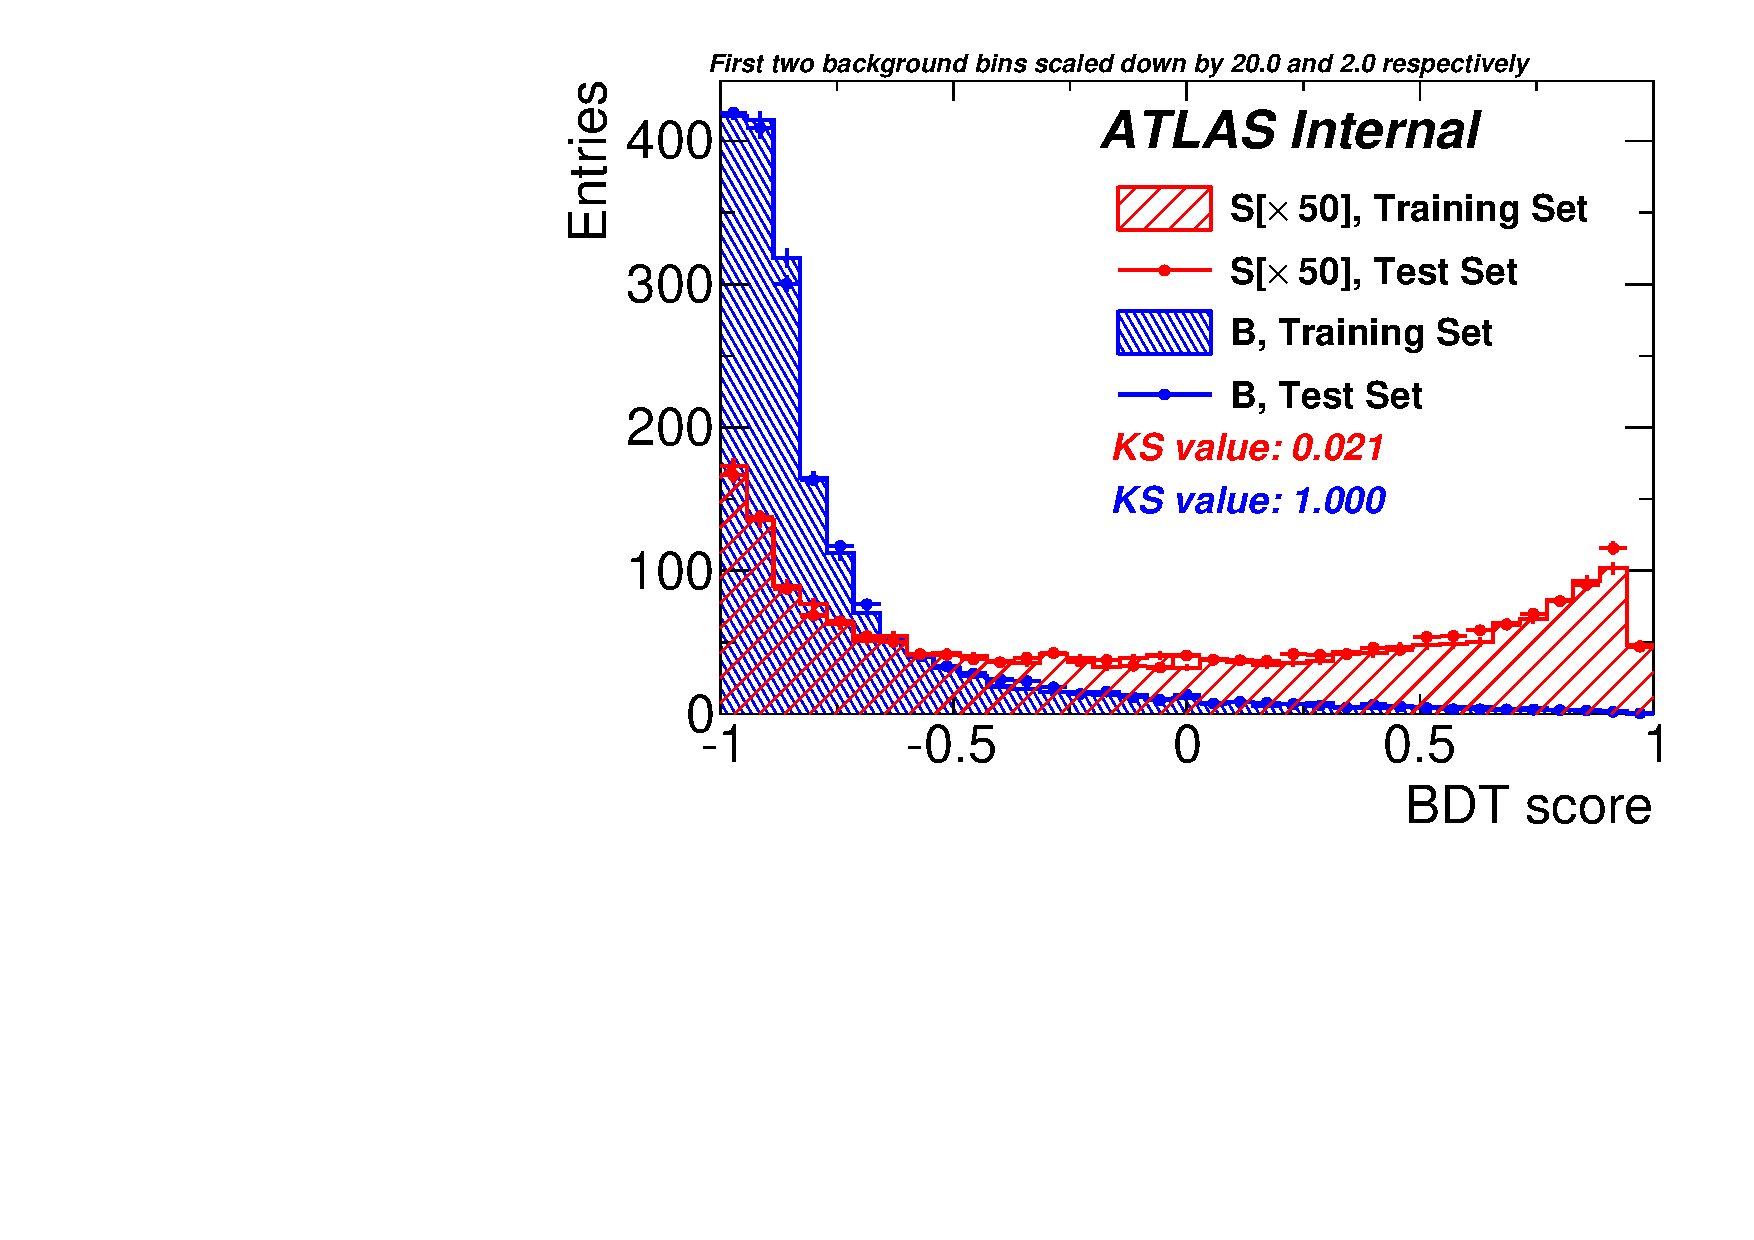
\includegraphics[width=0.49\textwidth]{bdt/overtraining_check1.pdf}
    \label{chap:bdt:fig:overtraining1}
    }
    \subfigure[Overtraining check for BDT 2]{
    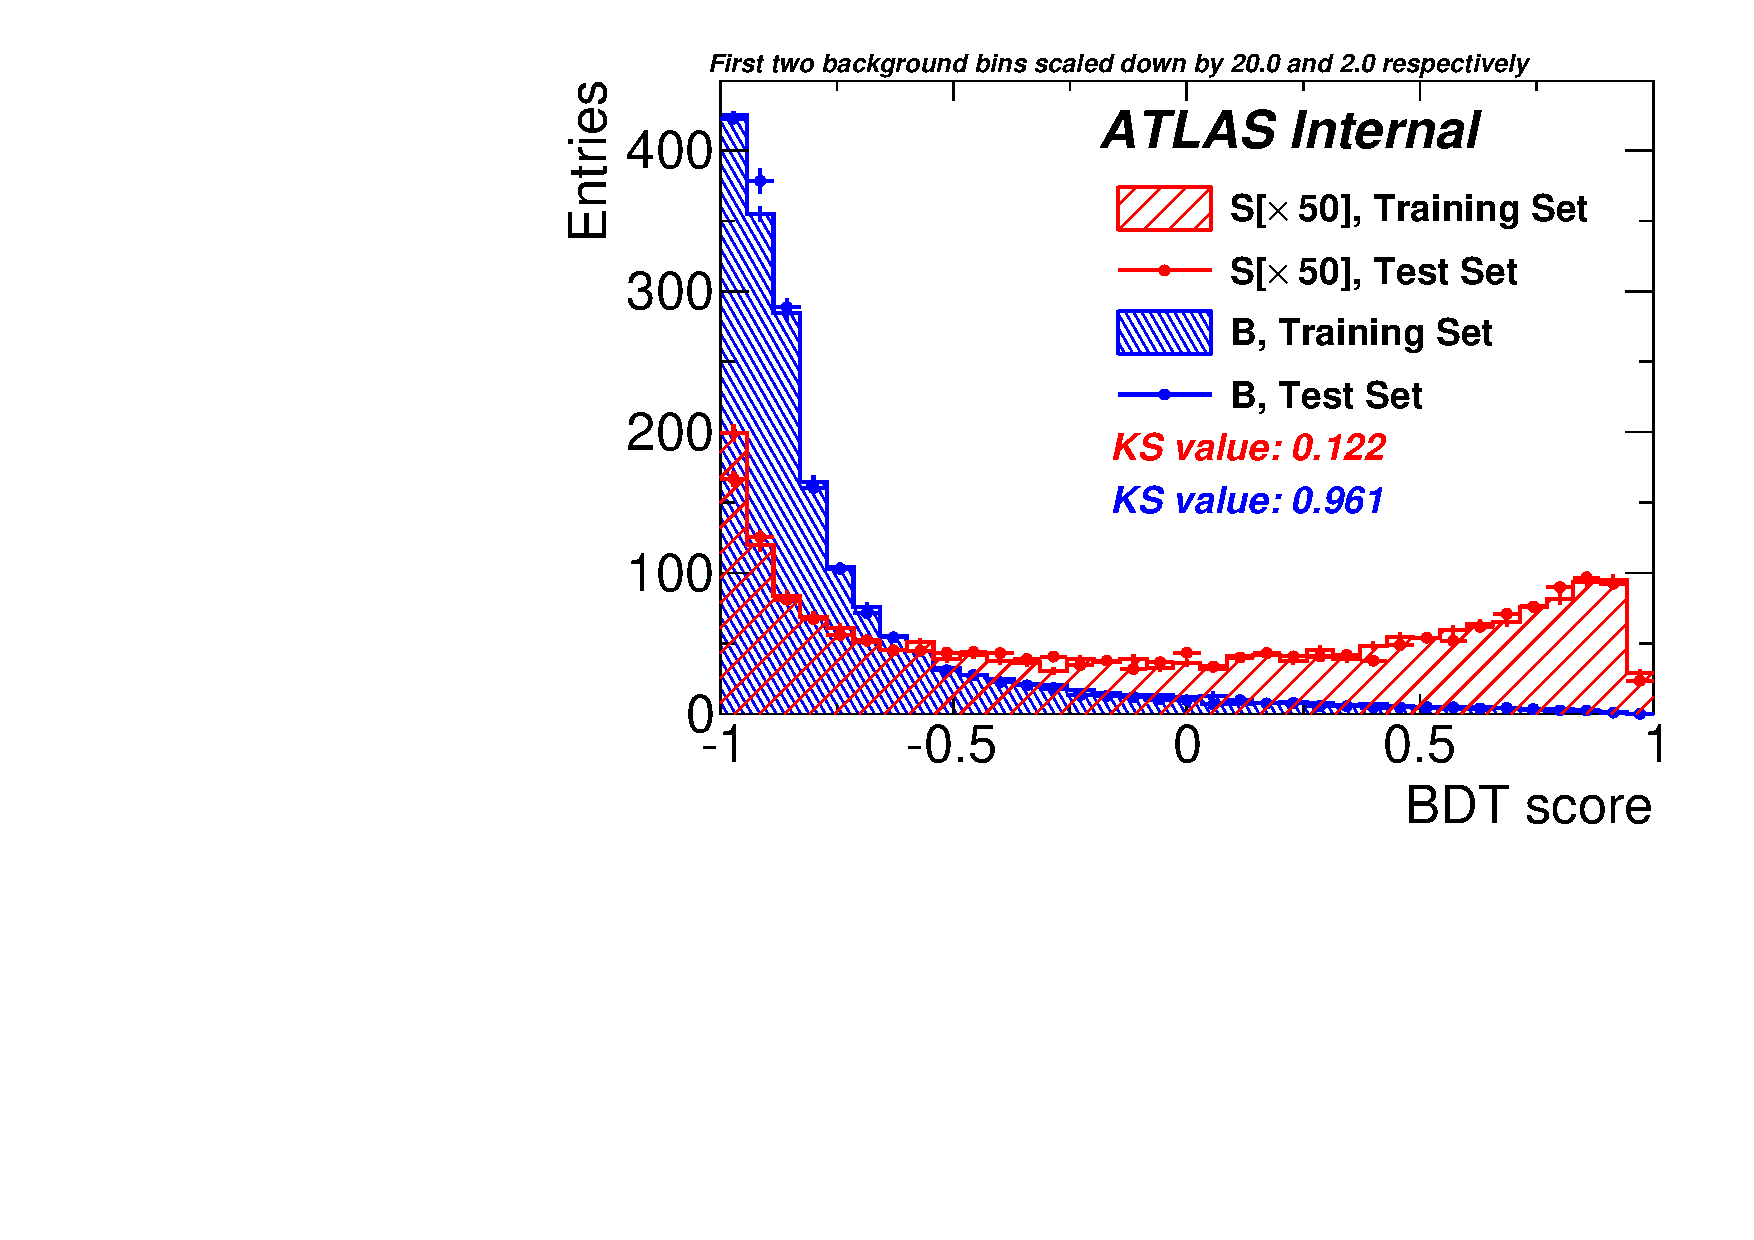
\includegraphics[width=0.49\textwidth]{bdt/overtraining_check2.pdf}
    \label{chap:bdt:fig:overtraining2}
    }
    \caption[Boosted decision tree overtraining check.]{Overtraining
      check for optimized boosted decision tree. Training set is shown
    in hatched distributions, while statistically independent test set
    is shown with points. First two background bins are scaled by 20.0
    and 2.0, respectively. Signal normalization multiplied by a factor
    of 50.}
\label{chap:bdt:fig:overtraining}
\end{figure}
